\documentclass[spanish]{article}

%%%%%%%%%%%%%%%%%%%%%%%%%%%%%%%%%%%%%%%%%%%%%%%%%%%%%%%%%%%%%%%%%%%%%%%%%%%%%%%%

% Language
\usepackage[spanish]{babel}

% Support for images
\usepackage{graphicx}

% Underlining
\usepackage{amsmath}

% Avoiding indenting of first paragraph's line.
\setlength{\parindent}{0cm}

% Support for hyperlinks.
\usepackage{hyperref}
\hypersetup {
        linktoc=all,
        hidelinks
}

% Additional section formatting.
\renewcommand\thesection{\arabic{section}}
\renewcommand\thesubsection{\thesection.\arabic{subsection}}

% Cover of the document
\title{Redes y Aplicaciones Internet - PEC 2}
\author{Oussama Akachach Jouhrati\\
[0.5cm]{\small Profesor/a: Maria Isabel March Hermo}}
\date{\today}

%%%%%%%%%%%%%%%%%%%%%%%%%%%%%%%%%%%%%%%%%%%%%%%%%%%%%%%%%%%%%%%%%%%%%%%%%%%%%%%%

\begin{document}

\pagenumbering{gobble}
\maketitle
\newpage

\tableofcontents
\pagenumbering{arabic}
\setcounter{page}{2}
\newpage


% Customize from here.

\section{Pregunta 1}

\subsection{Apartado a}

HTML es un lenguaje de marcado, en el que utilizan etqiuetas
para marcar texto plano que se convertirá en hipertexto..\\

HTTP es un protocolo para enviar páginas de hipertexto de un
servidor web a un navegador web.

\subsection{Apartado b}

En un protocolo sin estado, en la operación de petición del
cliente y la respuesta del servidor, este no necesita
retener ningún tipo de información sobre la sesión o el
estado de los dos intervinientes para futuras peticiones.\\

Un ejemplo de protocolos sin estado serían HTTP, UDP o
DNS.\\

En un protocolo con estado, el servidor sí que requiere
guardar información sobre el estado y la sesión.\\

Un ejemplo de protocolos con estado serían FTP y Telnet.

Las transacciones de protocolos sin estado suelen ser más
rápidas, simples y fáciles de implementar, mientras que las
transacciones de protocolos con estado suelen ser más
lentas, complejas y difíciles de implementar en Internet.\\

Además, son más difíciles de escalar a nivel de arquitectura
y, para procesar cada petición, se debe utilizar el mismo
servidor.

\subsection{Apartado c}

GET se utiliza para recibir datos de un recurso específico,
tiene una cabecera de datos y un cuerpo de datos.\\

HEAD funciona casi de la misma manera que GET, pero no tiene
cuerpo de respuesta. Esta sirve para verificar que una
petición de tipo GET devolvería datos, sin comprometerse a
la descarga total.

\subsection{Apartado d}

La diferencia entre una petición GET normal y una petición
GET condicional es que en la primera, en caso de que se haya
modificado el recurso a recibir durante el tiempo de la
petición y la respuesta, esta seguirá siendo la que recibió
el servidor proxy.\\

En una petición GET condicional, si el servidor proxy
detecta que hay una versión maś reciente del recurso, este
puede enviar un error 304 como respuesta, o enviar el
recurso actualizado.

\subsection{Apartado e}

En las conexiones persistentes, el servidor deja abierta la
conexión al enviar la respuesta, mientras que en las no
persistentes, se debe crear una conexión por cada objeto que
se envía, ya que una vez se envían los datos, la conexión se
cierra y nada se puede enviar posteriormente.

\section{Pregunta 2}

En el protocolo HTTP, las cookies sirven para que el
servidor pueda identificar las peticiones de un cliente y
ofrecer un servicio personalizado en sus respuestas.\\

Inicialmente, cuando un cliente realiza una petición HTTP a
un servidor, si esta no va acompañada de una cookie, el
servidor generará una para ese cliente específico, la
enviará junto con la respuesta y el navegador del cliente
almacenará dicha información.\\

Posteriormente, cuando el mismo cliente continúe efectuando
peticiones al servidor, este podrá reconocer al cliente
mediante la cookie y realizar acciones específicas, como por
ejemplo, ofrecer productos de venta de una manera más
personalizada, basada en las preferencias del/la usuario/a,
según sus hábitos de navegación por la web, debido a que
cada interacción que se hace con la página, va precedida de
una petición HTTP al servidor con el identificador de cookie
asignado.

\section{Pregunta 3}

SMTP es un protocolo TCP que se usa para enviar y recibir
correo. La comunicación entre el cliente, que es el programa
de correo del remitente, y el servidor, que es el servidor
de correo recibido del destinatario, se realiza mediante
comandos de texto plano.\\

POP es un protocolo TCP en el cual nos descargamos el correo
del servidor del destinatario.\\

IMAP funciona como el protocolo POP, pero la diferencia es
que este se descarga el correo cuando nosotros lo
solicitamos, mientras que el protocolo POP se descarga el
correo al tener conexión a internet.\\

\newpage

Las principales diferencias que hay entre estos protocolos
son las acciones a realizar: SMTP es un protocolo que sirve
para enviar correos del remitente, al servidor del
remitente, y luego al servidor del destinatario, mientras
que POP e IMAP sirven para recibir los correos, puesto que
se los descargan del servidor del destinatario.\\

En cuanto a puertos, SMTP funciona en el puerto 25, POP
funciona en el puerto 110 e IMAP funciona en el puerto
143.\\

En cuanto a estados, SMTP es un protocolo sin estado,
mientras que POP e IMAP son protocolos con estado.

\section{Pregunta 4}

\begin{center}

\includegraphics[width=12cm]{../img/2.png}
\end{center}

\textbf{Date:} Indica la fecha a la que se ha enviado el
mensaje.\\

\textbf{To:} Indica la dirección de correo del
destinatario.\\

\textbf{From:} Indica la dirección de correo del
remitente.\\

\textbf{Subject:} Indica el asunto del mensaje.\\

\textbf{Message-ID:} Se trata de un identificador del
mensaje, generado automáticamente.\\

\textbf{MIME-Version:} Indica la versión de MIME
(Multipurpose Internet Mail Extensions), la cual permite
añadir archivos adjuntos a un correo electrónico.\\

\textbf{Content-Type:} Indica el tipo de format odel cuerpo
del mensaje.

\section{Pregunta 5}

Explica la arquitectura de servidores DNS donde se muestren
los diferentes tipos de servidores y los dos tipos de
comunicación que puede haber entre ellos.

La arquitectura de los servidores DNS es jerárquica, es
decir, existen niveles a partir de los cuales se controla el
nivel inferior. Comenzando desde la raíz, formada por 13
servidores repartidos geográficamente, a partir de los
cuales se realiza la resolución inicialmente.\\

Seguido de este nivel, encontramos los dominios de nivel
superior, aquí encontraremos dominions como .com, .es, .net,
etc.\\

Después, encontramos los dominios de segundo nivel, que son
los nombres de las páginas que conocemos, como por ejemplo
amazon, netflix, google, etc.\\

Más adelante, encontramos los dominios de tercer nivel, que
pueden ser mail, www, etc.\\

Los niveles se separan por puntos, y el nivel superior
controla la resolución de su inferior, es decir, que google,
controlaría la resolución del dominio mail.google, para
acceder a GMail, por ejemplo.\\

Cuando se realiza una consulta DNS, siempre y cuando no
existe información almacenada en caché, los diferentes
tipos de servidores DNS trabajan conjuntamente para
completar la tarea de devolver la dirección IP de un dominio
específico al cliente. Todos los servidores DNS entran en una de estas cuatro
categorías:\\

\textbf{Recursive resolvers:} Actúa como intermediario entre
un cliente y un DNS nameserver. Este, al recibir una
petición por parte del cliente, responderá con datos
almacenados en caché, o enviará una petición al root
nameserver, seguido de una petición al TLD nameserver y,
finalmente, al authoritative nameserver. Tras recibir la
respuesta de éste, el recursive resolver enviará la
respuesta al cliente.\\

\textbf{Root nameservers:} Son la primera parada de un
recursive resolver. Existen 13 tipos de root nameservers y todos los
recursive resolvers tienen acceso a ellos. Al recibir la
petición del recursive resolver, este lo dirige a un TLD
nameserver, basado en la extensión del dominio o el dominio
de nivel superior.\\

\textbf{TLD nameservers:} Mantiene información de todos los
dominios que compartan una extensión o dominio de nivel
superior. Al recibir el TLD nameserver, un recursive
resolver enviaría una consulta al TLD nameserver
correspondiente, que le respondería con la dirección del
authoritative nameserver para ese dominio.\\

\textbf{Authoritative nameservers:} Suele ser el último paso
en la tarea de la búsqueda de una dirección IP. Este
contiene toda la información específica al dominio que
sirve.\\

Existen dos tipos de comunicación entre servidores DNS, DNS
over TLS y DNS over HTTPS.\\

\textbf{DNS over TLS:} Se trata de un estándar que sirve
para encriptar consultas DNS. Este tipo de comunicación
añade encripción TLS por encima del user datagram protocol,
que se usa para hacer consultas DNS.\\

\textbf{DNS over HTTPS:} Mediante este método, las consultas
DNS están encriptadas, pero se envían a través de protocolos
HTTP o HTTP/2, en lugar de UDP. De esta manera, se puede
asegurar que los atacantes no pueden alterar el tráfico DNS.

\section{Pregunta 6}

\subsection{Apartado a}

El tiempo de respuesta ha sido de 45 milisegundos.

\subsection{Apartado b}

Utiliza HTTP como protocolo de transporte.

\subsection{Apartado c}

Los flags activados son: qr, rd y ra.\\

\textbf{QR:} Indica que el mensaje es una consulta, con un
valor de 0, o una respuesta, con un valor de 1.\\

\textbf{RD:} Significa ``Recursion Desired'' e indica que es
una consulta recursiva.\\

\textbf{RA:} Significa `` Recursion Available'' e indica si
la recursion está disponible.

\subsection{Apartado d}

Hay cuatro registros A. Esto es debido a que el dominio
uoc.edu tendrá más de una dirección IP desde la cual se
puede acceder.

\newpage

\subsection{Apartado e}

Los nombres de servidores son:

\begin{enumerate}
\item ns-1939.awsdns-50.co.uk\\
\item ns-1305.awsdns-35.org\\
\item ns-611.awsdns-12.net\\
\item ns-68.awsdns-08.com\\
\end{enumerate}

La razón por la que hay varios es debido a que, dependiendo
del lugar en el que estemos, será más rápido cargar la
página en un servidor o en otro, según la distancia a la que
estemos de éste.\\

También es posible que cada servidor esté pensado para una
tarea de intercambio de datos específica. Podemos tener un
servidor que se encargue del manejo del correo electrónico,
otro que se encargue de desplegar la página, etc.

\subsection{Apartado f}

Sirve para poder ver todos los diferentes pasos que se
realizan en la resolución de DNS, es decir, cómo los
diferentes servidores se comunican entre sí para dar
respuesta a la consulta de una dirección IP através de un
dominio.\\

Primero, se hace una consulta de la raíz, que es la sección
superior de toda la jerarquía DNS. Seguido de ello, se busca
el dominio de nivel superior, en este caso, edu. Después, se
busca el dominio de segundo nivel, que en este caso, es uoc.
Por último, se busca el dominio de tercer nivel, que en este
caso,es w.\\

Una vez obtenemos la respuesta de la consulta en su
totalidad, se realizan los pasos ya vistos en la consulta
anterior, sin marcar la opción Trace.

\subsection{Apartado g}

El servidor de correo de un dominio requiere una consulta de
tipo MX o mail exchange.\\

El servidor de correo del dominio es
ns-1939.awsdns-50.co.uk.

\section{Pregunta 7}

Dentro de BitTorrent, existe una red virtual de usuarios/as,
através de los cuales se envían y reciben archivos que se
encuentren en el ordenador de uno/a o de varios/as
usuarios/as.\\

Cuando un/a usuario/a se descarga un archivo, este/a lo
recibe en bits que vienen de múltiples ordenadores que ya
tienen el archivo.\\

En resumen, este protocolo sirve para compartir archivos
mediante una red de ordenadores.

\section{Pregunta 8}

Con tal de evitar esperas, bufferings eternos y caídas del
sistema por colapsos, Netflix emplea una estrategia en la
que se reduce el número de canales por los que tiene que
pasar el contenido desde que se solicita, hasta que llega al
cliente (espectador/a). Esta consiste en tener servidores
con el contenido a visualizar tan cerca como sea posible del
cliente, a veces, dentro de las propias instalaciones el
proveedor de servicios de Internet que hayamos contratado.\\

Netflix tiene 17.000 servidores, repartidos en 158 países, y
tienen intención de continuar expandiéndose. El criterio que
utilizan para colocar los servidores está basado en las
ubicaciones donde hay la mayor parte de suscriptores y donde
estén los proveedores de servicios de Internet.\\

La diferencia entre la CDN de Netflix y la de otros
servicios es que su función es únicamente para servir los
intereses de Netflix, sin proveer de servicios a ninguna
otra compañía.\\

Los contenidos se replican mediante subidas periódicas a
todos los servidores de Netflix pero, con tal de evitar una
pérdida de ancho de banda necesario para los/as usuarios/as,
esta operación se realiza fuera de las horas de mayor
tráfico de red.\\

\newpage

\section{Pregunta 9}

Los tipos de plataformas para proporcionar servicios cloud
más representativas que aparecen en el módulo ``Fundamentos
y plataformas de cloud computing'' son:

\begin{enumerate}
\item Hipervisores o monitores de máquina virtual.
\item IaaS (infraestructura como servicio)
\item PaaS (plataforma como servicio)
\item SaaS (software como servicio)
\item StaaS (Almacenamiento como servicio)
\item NaaS (Red como servicio)
\end{enumerate}

Las dos plataformas escogidas son: PaaS (plataforma como
servicio) y SaaS (software como servicio).\\

La diferencia entre ellos consiste en que para un PaaS, se
nos provee de un servicio de herramientas de hardware y
software, las cuales son utilizadas por programadores,
mientras que en un SaaS, la aplicación ya existe y los
usuarios acceden a ella mediante una conexión a internet.\\

Un ejemplo de Saas sería Netflix. Se trata de un servicio
que ofrece visualización mediante streamign de películas o
vídeos. Utiliza un modelo de suscripciones donde el usuario,
según lo que pague accede a una calidad de vídeo y un número
de sesiones simultáneas.\\

Actualmente, existe una membresía en la cual no todo el
contenido está accesible, pero se paga menos. Para el resto
de categorías, todo el contenido del servicio está
disponible, pero no se tiene control sobre lo que se añade,
o se elimina.\\

Un ejemplo de PaaS sería SAP Cloud. Se trata de una
plataforma que permite a desarrolladores crear aplicaciones
de una manera más senzilla y permite la integración de otras
aplicaciones a la que se esté desarrollando.

\newpage

\section{Pregunta 10}

Busca información de dos ejemplos reales de servicios web
implementados con REST.\\

Para el primer ejemplo, en la página ``REST client'' de
postman.com, podemos ver que para que el navegador reciba el
documento HTML con el contenido de la página, se efectúa una
petición de tipo HTTP, mediante un servicio REST. El tipo de
petición es de tipo GET, donde se está solicitando un
archivo o datos.\\

Para el segundo ejemplo, en la página ``geeksforgeeks.org'',
podemos ver que para que el navegador reciba la imagen .jpg
del tutorial de python, se efectua una petición de tipo
HTTP, mediante un serivcio REST. El tipo de petición es de
tipo GET, también, pero en este caso, en lugar de pedir un
documento html, se pide un archivo .jpg.

\begin{center}
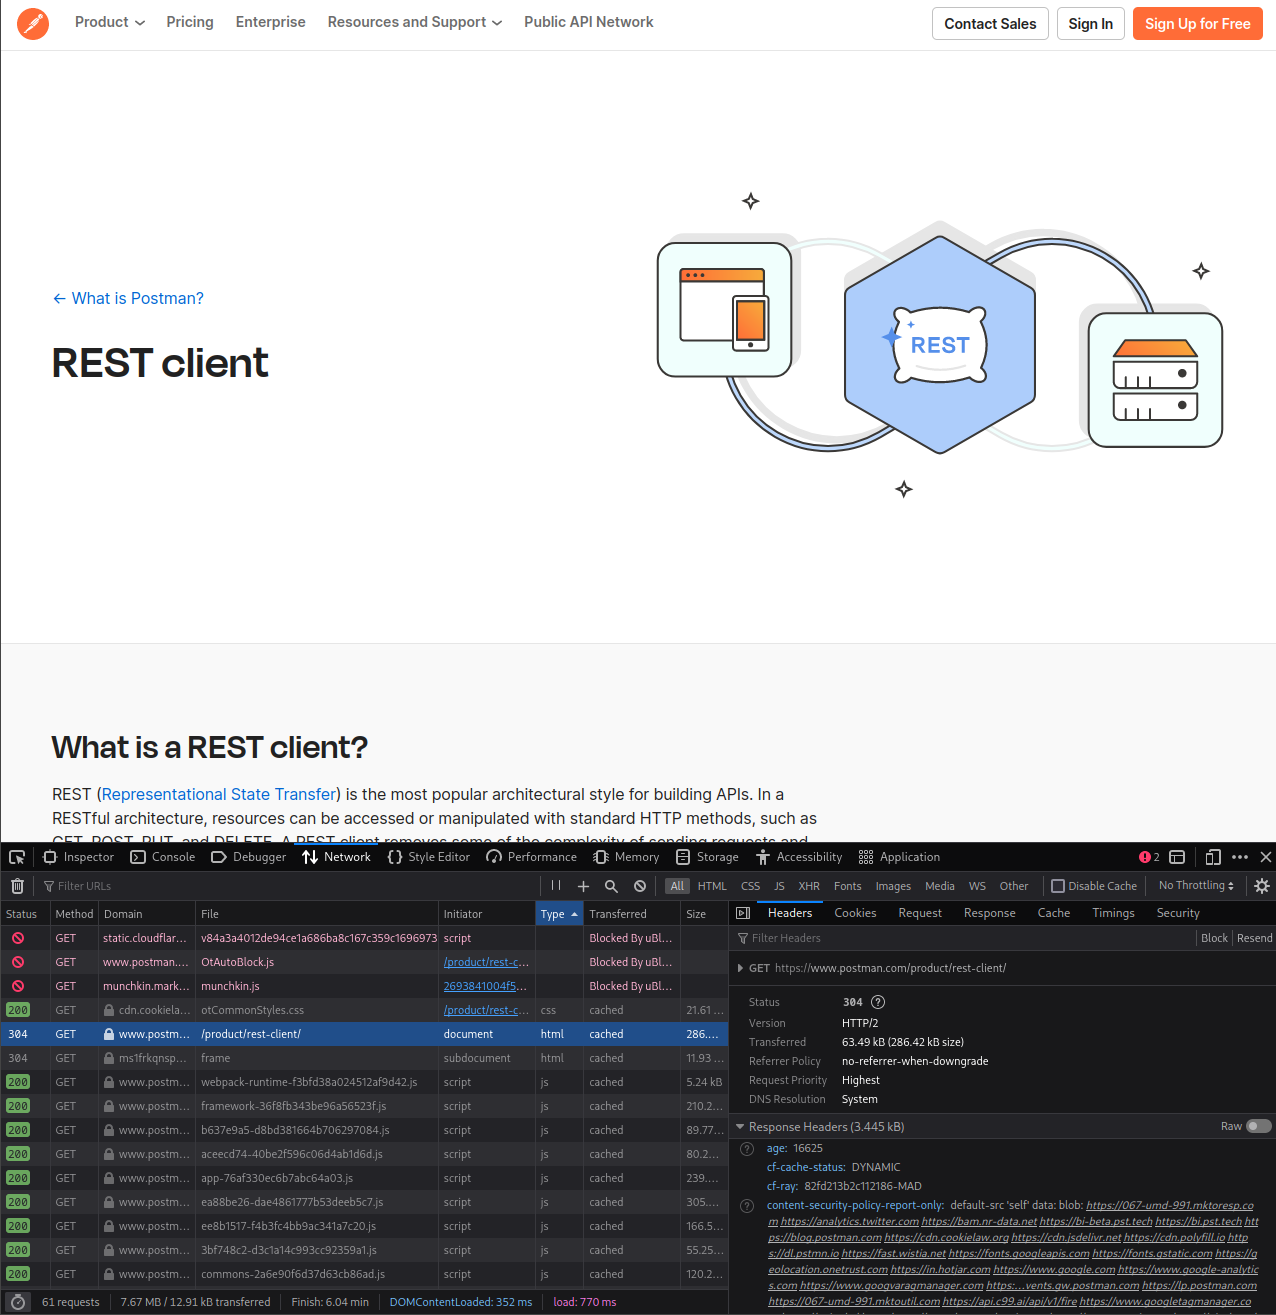
\includegraphics[width=12cm]{../img/1.png}
\end{center}

Otro mecanismo que sirve para implementar servicios web,
aparte de REST, es SOAP.\\

Significa Simple Object Access Protocol y consiste en un
documento XML separado por los siguientes apartados:

\begin{enumerate}
\item Un elemento raíz, llamado Envelope.
\item La cabecera o header, donde aparece la información de
enrutación del cliente al que le debe llegar la información.
\item El cuerpo o body, donde aparece el mensaje a enviar.
\end{enumerate}

Otro tipo de servicio web es GraphQL, el cual está basado en
un archivo JSON donde se escriben todas las posibles
consultas y los diferentes tipos de valores de retorno.\\

Y un último ejemplo sería WebSockets, donde se realiza la
comunicación sobre una sola conexión TCP.

\newpage

\begin{thebibliography}{X}

\item Monaselidze, G. (2023, May 9). Email headers
explained: Definition, components, role [2023].
\textit{Mailtrap.} https://mailtrap.io/blog/email-headers/\\

\item GeeksforGeeks. (2023, September 28). \textit{IMAP vs
POP3 vs SMTP.}
https://www.geeksforgeeks.org/imap-vs-pop3-vs-smtp/\\

\item GeeksforGeeks. (2019, August 8). \textit{Web caching
and conditional GET statements.}
https://www.geeksforgeeks.org/web-caching-and-conditional-get-statements/\\

\item GeeksforGeeks. (2023a, March 30). \textit{HTTP non
persistent Persistent Connection Set 1.}
https://www.geeksforgeeks.org/http-non-persistent-persistent-connection/\\

\item \textit{HTTP Methods GET vs POST.} (n.d.).
https://www.w3schools.com/tags/ref\_httpmethods.asp\\

\item GeeksforGeeks. (2022, November 2). \textit{Difference
between HTML and HTTP.}
https://www.geeksforgeeks.org/difference-between-html-and-http/\\

\item Khan, B. (2020, August 8). \textit{DNS explained.
Hierarchy and architecture.} DEV Community.
https://dev.to/blake/dns-explained-hierarchy-and-architecture-18pj\\

\item Cloudflare. (2023, November 27). \textit{DNS server
types.}
https://www.cloudflare.com/learning/dns/dns-server-types/\\

\item Cloudflare. (2023, Novembre 27). \textit{DNS over TLS
vs. DNS over HTTPS | Secure DNS}.
https://www.cloudflare.com/learning/dns/dns-over-tls/\\

\item Ns. (2022, January 25). \textit{Using dig +trace to
Understand DNS Resolution from Start to Finish.} NS1. https://ns1.com/blog/using-dig-trace

\item GeeksforGeeks. (2023, July 23). \textit{What is P2P 
Peer to Peer Process.} https://www.geeksforgeeks.org/what-is-p2p-peer-to-peer-process/

\item Team, P. (2023, November 16). \textit{A guide to the
different types of APIs.} Postman Blog. https://blog.postman.com/different-types-of-apis/

\item GeeksforGeeks. (2023a, January 17). \textit{Difference
between IAAS  PAAS and SAAS.} https://www.geeksforgeeks.org/difference-between-iaas-paas-and-saas/

\item Shim, T. (2023, April 19). \textit{15 Popular Platform as a
Service (PAAS) examples.} Web Hosting Secret Revealed (WHSR).
https://www.webhostingsecretrevealed.net/blog/web-business-ideas/paas-examples/\#2-sap-cloud 
\end{thebibliography}

\end{document}
